\documentclass[default]{subfiles}

\addbibresource{cite.bib}

% Fill in every \PH{...} item before submitting: search for TODO in the compiled PDF.
\providecommand{\PH}[1]{\textbf{[TODO: #1]}}

\begin{document}

{%
\selectlanguage{english}

\udc{004.8, 004.62}

\pacs{%
  07.05.Kf, %Data analysis: algorithms and implementation; data management
  07.05.Mh %Neural networks, fuzzy logic, artificial intelligence
}

\edn{xxxxxx}

\documentType{Research article}

\title{Fragile Reference Answers on Real Data: An Audit of the EMT Madrid Open Parking Dataset for Evaluating Language Models and AI Agents}

\author[urfu]{Tamerlan M. Kizilbaev}
\author[urfu]{Timofey V. Novikov}
\author[urfu]{Kirill V. Bagin}
\author[urfu]{Egor E. Golovin}
\author[urfu]{Rolan R. Balapanov}

\address[urfu]{Institute of Radioelectronics and Information Technologies -- RTF, Ural Federal University named after the first President of Russia B. N. Yeltsin, 19 Mira St, Yekaterinburg, 620002, Russian Federation}

\begin{authordescription}
  \authorfull[english]{Kizilbaev, Tamerlan M.}
  \authorpost[english]{Student of the Institute of Radioelectronics and Information Technologies -- RTF, Ural Federal University}
  \email{kizilbaev06@mail.ru}
  \orcid{0009-0005-6097-2623}
\end{authordescription}

\begin{authordescription}
  \authorfull[english]{Novikov, Timofey V.}
  \authorpost[english]{Student of the Institute of Radioelectronics and Information Technologies -- RTF, Ural Federal University}
  \email{timofie8456@gmail.com}
  \orcid{0009-0001-3885-7697}
\end{authordescription}

\begin{authordescription}
  \authorfull[english]{Bagin, Kirill V.}
  \authorpost[english]{Student of the Institute of Radioelectronics and Information Technologies -- RTF, Ural Federal University}
  \email{kirilbagin@yandex.ru}
  \orcid{0009-0007-5242-3485}
\end{authordescription}

\begin{authordescription}
  \authorfull[english]{Golovin, Egor E.}
  \authorpost[english]{Student of the Institute of Radioelectronics and Information Technologies -- RTF, Ural Federal University}
  \email{egorgolovin75@gmail.com}
  \orcid{0009-0003-3172-1951}
\end{authordescription}

\begin{authordescription}
  \authorfull[english]{Balapanov, Rolan R.}
  \authorpost[english]{Student of the Institute of Radioelectronics and Information Technologies -- RTF, Ural Federal University}
  \email{chipavoyvoy@gmail.com}
  \orcid{0009-0004-0889-7323}
\end{authordescription}

\abstracts{%
\textbf{Background:} Large language models (LLMs) and AI agents are compared on benchmarks that assume the reference answer is correct and unambiguous. On real open data this is not guaranteed: a reference computed by a formal rule may reproduce a measurement defect. \textbf{Aims:} To quantify how measurement defects and unstated computational conventions change reference answers, and to propose and test an evaluation protocol that accounts for these effects. \textbf{Materials and Methods:} We audited an open hourly parking dataset of Empresa Municipal de Transportes de Madrid (EMT) for May--September 2026 (301,104 rows) and a package of 85 reference answers, using independent recalculation, a frozen-reading detector, sensitivity analysis, and coverage control. Three LLMs then answered all 85 questions without tools and as code-executing agents, with the package wording and with the protocol, and reviewed each file for defects (1,035 runs). \textbf{Results:} The package is technically reproducible, yet 64.6\% of rows hold a service value and 9.6\% of valid rows belong to frozen runs. Frozen sensors create an apparent June peak in capacity-weighted occupancy (63.8\% versus 52.8\% after cleaning) and determine the ``busiest car park'' answer. Rounding to four decimals breaks 25 of 40 fractional references, and the outlier counts depend on the quartile method and on floating-point rounding; two of them differ from the exact value. Agents answered 71--85 of 85 questions correctly, models without tools 5--10. Strict comparison rejected exactly the 25 predicted correct answers of every agent, and all 34 agent errors were either missing answers or tied to the outlier question and an ambiguous rule wording. In open reviews the agents found 19--43 of 43 known defects. \textbf{Conclusions:} A reference without stated conventions and measurement checks partly scores systems on incidental features. We propose a protocol with explicit conventions, an adjusted tolerance, dual references, and separate scoring of defect detection.
}

\keywords{large language models, AI agents, tabular data analysis, benchmarks, data quality, reproducibility, open data, sensor faults}

\alttitle{Хрупкие эталоны на реальных данных: аудит открытого набора о парковках EMT Madrid для оценки языковых моделей и ИИ-агентов}

\altauthor[urfu]{Т. М. Кизильбаев}
\altauthor[urfu]{Т. В. Новиков}
\altauthor[urfu]{К. В. Багин}
\altauthor[urfu]{Е. Е. Головин}
\altauthor[urfu]{Р. Р. Балапанов}

\altaddress[urfu]{Институт радиоэлектроники и информационных технологий -- РтФ, Уральский федеральный университет имени первого Президента России Б. Н. Ельцина, ул. Мира, д. 19, Екатеринбург, 620002, Российская Федерация}

\altabstracts{Большие языковые модели (LLM) и ИИ-агенты сравнивают по эталонным наборам, предполагая, что эталонный ответ верен и однозначен. На реальных открытых данных это не гарантировано: эталон, рассчитанный по формальному правилу, может воспроизводить дефект измерения. Цель работы — оценить, насколько дефекты измерений и незафиксированные вычислительные соглашения меняют эталонные ответы, предложить протокол оценки, учитывающий эти эффекты, и проверить его. Проведен аудит открытого набора почасовых данных о парковках Empresa Municipal de Transportes de Madrid (EMT) за май–сентябрь 2026 г. (301 104 строки) и пакета из 85 эталонных ответов: повторный и независимый расчет, детектор застывших показаний, анализ чувствительности эталонов и контроль покрытия. Затем три LLM ответили на все 85 вопросов без инструментов и в роли агентов с выполнением кода, в формулировке пакета и по протоколу, а также проверили каждый файл на дефекты (1035 запусков). Пакет технически воспроизводим, однако 64,6 \% строк содержат служебное значение, а 9,6 \% допустимых строк относятся к застывшим отрезкам. Застывшие датчики создают кажущийся пик взвешенной занятости в июне (63,8 \% против 52,8 \% после очистки) и определяют ответ о самой загруженной парковке. Округление до четырех знаков нарушает 25 из 40 дробных эталонов, а счетчики выбросов зависят от метода квартилей и от округления в арифметике с плавающей точкой; два из них расходятся с точным значением. Агенты верно ответили на 71–85 из 85 вопросов, модели без инструментов — на 5–10. Строгое сравнение отвергло у каждого агента ровно 25 предсказанных верных ответов, а все 34 ошибки агентов — это отсутствие ответа либо вопрос о выбросах и неоднозначная формулировка правила. При открытой проверке файлов агенты нашли от 19 до 43 из 43 известных дефектов. Эталон без зафиксированных соглашений и проверки измерений оценивает систему частично по случайным признакам. Предложен протокол с явными соглашениями, скорректированным допуском, двойным эталоном и отдельной оценкой обнаружения дефектов.}

\altkeywords{большие языковые модели, ИИ-агенты, анализ табличных данных, эталонные наборы, качество данных, воспроизводимость, открытые данные, неисправности датчиков}

\maketitle

\section{Introduction}

Large language models (LLMs) are increasingly used to analyse tables: counts, descriptive statistics, grouping, and anomaly search. AI agents, here meaning LLM-based systems that can execute code and work with files, can compute exactly even on tables that do not fit into the model context. Such systems are compared on benchmarks in which each table and question comes with a correct answer and a tolerance~\cite{lai2023,hu2024,huang2024,jing2024}.

It is usually assumed that the reference answer is correct and unambiguous. For real open data this is not guaranteed: they contain service codes, transmission failures, sensors with frozen readings, and errors in reference fields. A reference computed by a formal rule may reproduce a measurement artifact, and a system that justifiably excludes the artifact is then scored as wrong. The answer also depends on conventions that questions do not always state: degrees of freedom, quantile method, and the form in which a share is written.

The effect of imperfect data on LLMs is already being studied, but mostly with artificially injected distortions and a known correct answer~\cite{gu2025,wolff2025}, while reference errors are studied as label errors or incorrect gold queries~\cite{northcutt2021,wretblad2024}. Less attention has been paid to the case in which a reference is computed without error yet inherits a natural measurement defect and unstated conventions. This paper examines that case using an open parking dataset of the Madrid municipal transport company (Empresa Municipal de Transportes de Madrid, EMT) and a package of 85 reference answers built on it.

The aim is to assess how robust reference answers are to measurement defects and computational conventions and to propose an evaluation protocol that accounts for these effects. Our contributions are as follows:

\begin{enumerate}
  \item we present a package that is fully reproducible technically yet contains references that describe measurement artifacts;
  \item we quantify the sensitivity of references to rounding, tolerance, the degrees-of-freedom correction, quantile method, and filtering;
  \item we apply a constant-reading detector to benchmark auditing and derive a cleaning variant, P1-S;
  \item we propose an evaluation protocol that separates answer accuracy from the ability to detect data defects;
  \item we test the protocol on three LLMs without tools and as code-executing agents and show which part of the measured error comes from the references and the wording rather than from the systems.
\end{enumerate}

\section{Related work}

\emph{Benchmarks for data analysis.} DS-1000 contains 1,000 problems across seven Python libraries collected from StackOverflow~\cite{lai2023}. InfiAgent-DABench includes 603 questions on 124 CSV files, converted to closed form for automatic scoring~\cite{hu2024}. DA-Code tests agent-based data work in Python and SQL~\cite{huang2024}, and DSBench combines data analysis and modelling tasks from competitions~\cite{jing2024}. Automatic scoring in such benchmarks relies on a known answer, so the reliability of that answer bounds the reliability of the evaluation.

\emph{Imperfect data.} RADAR contains 2,980 table--query pairs with five artifact types programmatically injected into real tables, and frontier models degrade significantly on them~\cite{gu2025}. Wolff and Hulsebos report degraded LLM reasoning under missing values and duplicate entities, and the unreliability of free-text metrics for such tasks~\cite{wolff2025}. DataGovBench is built from governmental open data and reports significant performance gaps, including with agent frameworks~\cite{hasegawa2026}. Unlike these works, the defects here are not injected: no clean version of the table exists, and the reference itself depends on a decision about what counts as a measurement.

\emph{Reliability of references.} Northcutt et al. found label errors in the test sets of 10 datasets and showed that they can change conclusions about model comparison~\cite{northcutt2021}. For text-to-SQL, incorrect gold queries were shown to weaken the reliability of BIRD-Bench and to change the relative standing of methods~\cite{wretblad2024}. Ambig-DS evaluates agents under ambiguous task framing~\cite{stoisser2026}, and the dependence of conclusions on the choice of benchmark is discussed in~\cite{dehghani2021}. The case considered here differs in that the reference contains no arithmetic error.

\emph{Data quality and sensor faults.} Methodologies for data quality assessment are systematised in~\cite{batini2009}. Sharma et al. distinguish three types of sensor faults, including constant readings (CONSTANT), and consider zero standard deviation within a window as a simple detection rule, noting that the result depends on window size~\cite{sharma2010}. Parking occupancy data are used in forecasting~\cite{stolfi2020}, which raises the cost of unnoticed defects.

\emph{Conventions and reproducibility.} The divergence of sample quantile definitions across statistical packages is described in~\cite{hyndman1996}; we show that for the outlier count under the 1.5 interquartile range rule~\cite{tukey1977} it changes an exact integer answer. The risk of test data entering LLM training sets is discussed in~\cite{sainz2023}, and leakage and reproducibility failures in machine-learning-based science in~\cite{kapoor2023}.

\section{Materials and methods}

\subsection{Source data}

We used the EMT series ``Plazas totales y disponibles por hora en aparcamientos por mes y año'', published on the EMT portal~\cite{emt} and in the Madrid open data catalogue~\cite{madrid} (the city catalogue states CC BY 4.0 and the EMT resource pages state ODC-By). We took five monthly files for May--September 2026, accessed on 14 October 2026, and recorded their SHA-256 checksums. The fields are listed in Table 1.

\begin{table}[htbp]
  \caption{Fields of the source files}
  \label{tab:1}
  \centering\small
  \begin{tabular}{p{\dimexpr 0.200\linewidth-2\tabcolsep\relax}p{\dimexpr 0.180\linewidth-2\tabcolsep\relax}p{\dimexpr 0.620\linewidth-2\tabcolsep\relax}}
    \hline
    \textbf{Field} & \textbf{Type} & \textbf{Content} \\ \hline
    dateServ & Date & Calendar date, YYYY-MM-DD \\
    hour & Integer & Hour label from 0 to 23; time zone and label meaning are not specified \\
    idParking & Identifier & Car park number, 82 values \\
    isEmtPark & Boolean & EMT flag: True for 31 car parks, False for 51 \\
    freeParking & Integer & Number of free spaces; includes the service value $-$1 \\
    parkingSpaces & Integer & Capacity, from 4 to 3,027 spaces; constant for each car park \\
    \hline
  \end{tabular}
\end{table}

The dataset contains 301,104 rows. The ``day $\times$ 24 hours $\times$ 82 car parks'' grid is complete, with no empty cells, duplicates, or conflicting keys. The files belong to one panel with the same set of car parks and are therefore not independent sources.

Reference answers were taken from a package comprising the source files, programs, result tables, and 85 reference values. The package was prepared by our project team on 14 October 2026, before the audit, for a planned comparison of LLMs and an agent, and is published in the project repository (see Data availability).

\subsection{Cleaning rule and occupancy measures}

The package's main rule, P1, treats a row as valid if all fields are parsed, the date belongs to the file's month, the hour lies between 0 and 23, the identifier and capacity are positive, and the number of free spaces is at least zero and at most the capacity. Zeros, statistical outliers, and constant readings are retained. The occupancy of a car park in a given hour is

\begin{equation}
  o = 1 - \frac{f}{c},
  \label{eq:o}
\end{equation}

where \emph{f} is the number of free spaces (field freeParking) and \emph{c} is the capacity (field parkingSpaces). The mean occupancy of a group of \emph{n} valid rows is computed in two ways: by rows, with every ``car park--hour'' record weighted equally, and weighted by capacity:

\begin{equation}
  O_r = \frac{1}{n}\sum_i o_i,
  \label{eq:r}
\end{equation}

\begin{equation}
  O_w = 1 - \frac{\sum_i f_i}{\sum_i c_i}.
  \label{eq:w}
\end{equation}

\subsection{Reference tasks}

The package defines 17 questions for each month, 85 reference answers in total, with an absolute tolerance of 10$^{-6}$ for fractional values. Table 2 groups the questions by the skill tested and gives for each group a trap in which a superficial solution yields a plausible but wrong answer.

\begin{table}[htbp]
  \caption{Categories of reference tasks}
  \label{tab:2}
  \centering\small
  \begin{tabular}{p{\dimexpr 0.220\linewidth-2\tabcolsep\relax}p{\dimexpr 0.400\linewidth-2\tabcolsep\relax}p{\dimexpr 0.380\linewidth-2\tabcolsep\relax}}
    \hline
    \textbf{Category} & \textbf{Metrics} & \textbf{Trap} \\ \hline
    File reading & data\_rows & Empty first line, header \\
    Quality control & minus1\_n, other\_negative\_n, above\_capacity\_n, valid\_n & $-$1 looks like a number; capacity overruns are easy to miss \\
    Descriptive statistics & free\_mean, free\_median, free\_std\_sample, free\_q1, free\_q3, free\_max & ddof correction, quantile method; median is $-$1 without a filter \\
    Derived measures & occupancy\_mean, occupancy\_capacity\_weighted & Substituting one mean for the other \\
    Grouping and maximum & peak\_hour\_all\_ties, peak\_hour\_mean\_occupancy, top\_parking\_all\_ties & Small margin, ties, faulty sensor \\
    Outlier detection & iqr\_flag\_n & 0 without grouping; quartile method changes the answer \\
    \hline
  \end{tabular}
\end{table}

\subsection{Reproducibility check}

We verified the checksums of all 27 files listed in CHECKSUMS.sha256 and the source hashes in the manifest. The package's calculation program was re-run and the results were compared byte by byte. The values were then recalculated with a separate program, audit\_repro.py.

\subsection{Detection of measurement defects}

In addition to the package's own checks, we applied a frozen-run detector, a variant of the constant-reading rule~\cite{sharma2010}. The valid rows of each car park are sorted by time; a run is a maximal sequence of identical numbers of free spaces. Invalid rows do not break a run, since $-$1 is treated as a missing measurement rather than a change. A run of at least \emph{L} = 24 valid hours is flagged as frozen. The cleaning variant P1-S is obtained from P1 by removing flagged rows; robustness to the threshold was checked at \emph{L} = 12.

\subsection{Sensitivity analysis and coverage control}

The reference metrics of each month were recalculated under deviations typical of LLM and agent answers: rounding to 2, 3, 4, and 6 decimals and writing shares as percentages; ddof = 0 instead of 1 in the sample standard deviation (SD); three quantile methods (linear interpolation, the ``exclusive'' method, and nearest rank; types 7, 6, and 1 in the classification of Hyndman and Fan~\cite{hyndman1996}); three alternative filters and no filtering; and counting outliers without grouping by car park. A reference is considered broken if the deviation exceeds its tolerance. All values in Tables 3--8 can be recomputed from the source files with the script audit\_repro.py (see Data availability).

Monthly occupancy dynamics were checked in four ways: (1) stable composition, 27 car parks excluding IDs 15, 49, and 80, equally weighted; (2) balanced panel, only the date-hours in which all 27 car parks are valid; (3) standardisation, the mean over ``day of week $\times$ hour'' cells for the same 27 car parks; (4) the P1-S cleaning variant. In addition, each car park's August occupancy was compared with its own mean over the other months.

\subsection{Experiment with LLMs and agents}

Three models were queried on 10--11 November 2026 through the OpenAI-compatible interface of a third-party gateway: Claude Sonnet 5.5 (Anthropic), GPT-6.1 Sol (OpenAI), and DeepSeek-V4-Pro (DeepSeek, version 0813). Each question was asked once at temperature 0.

In the \emph{LLM} mode the model received one request without tools containing the question, the number of data rows, the header, and the first 200 rows of the file. In the \emph{agent} mode the same model had two tools: a description of the table and the execution of model-written Python code with the pandas library in a separate process (60 s limit, output truncated to 8,000 characters, no access keys in the environment). An agent could make up to 12 requests; if it stopped without a final answer, it was reminded once.

Each of the 85 questions was asked under two conditions. Under the \emph{package} condition the question was preceded by the package's own processing rule, verbatim. Under the \emph{protocol} condition it was preceded by the conventions of item 1 of the protocol (see Evaluation protocol) and a request to answer under P1 and to name any defect that affects the answer. The answer had to end with the line ``ANSWER: value''. Answers were scored in three ways: with the package's tolerance (strict), by items 2--4 of the protocol, and with the P1-S alternative for occupancy and the busiest car park.

In addition, the agent was asked to review each monthly file for defects of measurements and reference fields and to give, for each defect, the car parks, its scale, and its effect on the means. An open review needs more steps, so this task allowed 20 requests and, if they ran out, one final request without tools. A first run with the question limit of 12 left 7 of 10 reports of Claude Sonnet 5.5 and DeepSeek-V4-Pro empty; these 7 were repeated, and the other 8 reports come from the first run. The 15 reports were scored against a checklist of 11 defects from Tables 3 and 5; 43 ``defect--month'' pairs are present in the data. Two annotators scored the reports independently, without knowing which model wrote each report, using written criteria for each defect, and also marked reports that contain false claims about defects.

\section{Results}

\subsection{Reproducibility of the package}

All 27 checksums and five source hashes matched. Re-execution on Python 3.10.11 (the package used 3.12.14) produced 10 of 14 files byte-identical to those in the package. In the other four, the differences are limited to the last digit of one SD value (3$\cdot$10$^{-14}$), the Python version string, and line endings. The separate recalculation matched the package for all compared metrics and months. Two limitations were found: the June and August files are confirmed by only one of the two official catalogues because the other timed out during the check, and the independent reconciliation program referenced by the package's validation file is missing from the archive.

\subsection{Defect profile}

The table has no empty cells but few measurements (Table 3). Almost two thirds of rows hold no measurement, and 48.4\% of spaces have no valid value at all. Monthly measures are given in Table 4.

\begin{table}[htbp]
  \caption{Data defects}
  \label{tab:3}
  \centering\small
  \begin{tabular}{p{\dimexpr 0.450\linewidth-2\tabcolsep\relax}p{\dimexpr 0.550\linewidth-2\tabcolsep\relax}}
    \hline
    \textbf{Defect} & \textbf{Scale} \\ \hline
    freeParking = $-$1 & 194,585 rows (64.6\%) \\
    Car parks with no valid values & 52 of 82; the 30 working car parks hold 13,342 of 25,833 spaces (51.6\%) \\
    Free spaces above capacity & 685 rows, 672 of them at ID 32 \\
    Values below $-$1 & 9 rows, all at ID 37 (from $-$1 to $-$12) \\
    Frozen runs of at least 24 h & 10,151 P1 rows (9.6\%) at six car parks \\
    Valid rows under P1 & 105,825 (35.1\%) \\
    \hline
  \end{tabular}
\end{table}

\begin{table}[htbp]
  \caption{Main monthly measures (rule P1)}
  \label{tab:4}
  \centering\small
  \begin{tabular}{p{\dimexpr 0.150\linewidth-2\tabcolsep\relax}p{\dimexpr 0.130\linewidth-2\tabcolsep\relax}p{\dimexpr 0.200\linewidth-2\tabcolsep\relax}p{\dimexpr 0.180\linewidth-2\tabcolsep\relax}p{\dimexpr 0.200\linewidth-2\tabcolsep\relax}p{\dimexpr 0.140\linewidth-2\tabcolsep\relax}}
    \hline
    \textbf{Month} & \textbf{P1 rows} & \textbf{Mean free spaces} & \textbf{Occupancy by rows, \%} & \textbf{Capacity-weighted occupancy, \%} & \textbf{Peak hour} \\ \hline
    May & 21,765 & 188.50 & 54.5 & 57.6 & 12 \\
    June & 21,050 & 161.05 & 53.7 & 63.8 & 12 \\
    July & 21,812 & 188.37 & 49.6 & 57.7 & 12 \\
    August & 20,556 & 232.74 & 44.4 & 47.1 & 13 \\
    September & 20,642 & 208.58 & 53.1 & 52.9 & 12 \\
    \hline
  \end{tabular}
\end{table}

June stands out: its capacity-weighted occupancy is about 6 percentage points (pp) above May and July, whereas occupancy by rows is almost the same in May and June.

\subsection{Frozen sensors}

The package's built-in check flags a car park only if all of its valid values in a month are identical. It finds IDs 15 and 49 in every month and ID 80 only in June. The run detector found 19 frozen runs at six car parks (Table 5).

\begin{table}[htbp]
  \caption{Frozen runs of at least 24 h}
  \label{tab:5}
  \centering\small
  \begin{tabular}{p{\dimexpr 0.080\linewidth-2\tabcolsep\relax}p{\dimexpr 0.200\linewidth-2\tabcolsep\relax}p{\dimexpr 0.320\linewidth-2\tabcolsep\relax}p{\dimexpr 0.180\linewidth-2\tabcolsep\relax}p{\dimexpr 0.220\linewidth-2\tabcolsep\relax}}
    \hline
    \textbf{ID} & \textbf{Value / capacity} & \textbf{Longest run} & \textbf{Period} & \textbf{Built-in check} \\ \hline
    15 & 0 / 394 & 3,494 h & whole period & Finds \\
    49 & 114 / 294 & 3,494 h & whole period & Finds \\
    80 & 0 / 3,027 & 1,282 h and 11 more runs & 20.05--14.07 & June only \\
    76 & 401 / 461 & 805 h, then 136 h at 400 & 20.05--29.06 & Misses \\
    79 & 113 / 359 & 88 h, and 24 h at 249 & 24.06--06.07 & Misses \\
    9 & 190 / 281 & 26 h & 06.06--08.06 & Misses \\
    \hline
  \end{tabular}
\end{table}

ID 80 is the largest car park, with 23\% of the capacity of working car parks. Its readings are doubtful throughout the period: of 3,494 valid values, 1,616 are zero, the other 1,878 lie between 1,611 and 1,719, and there are no values from 1 to 1,610 (Figure 1). The car park alternates between completely full and about 44\% occupied, and the zero run from 20 May to 14 July lasts 1,282 h. The absence of intermediate values points to a probable sensor failure.

\begin{figure}[htbp]
  \centering
  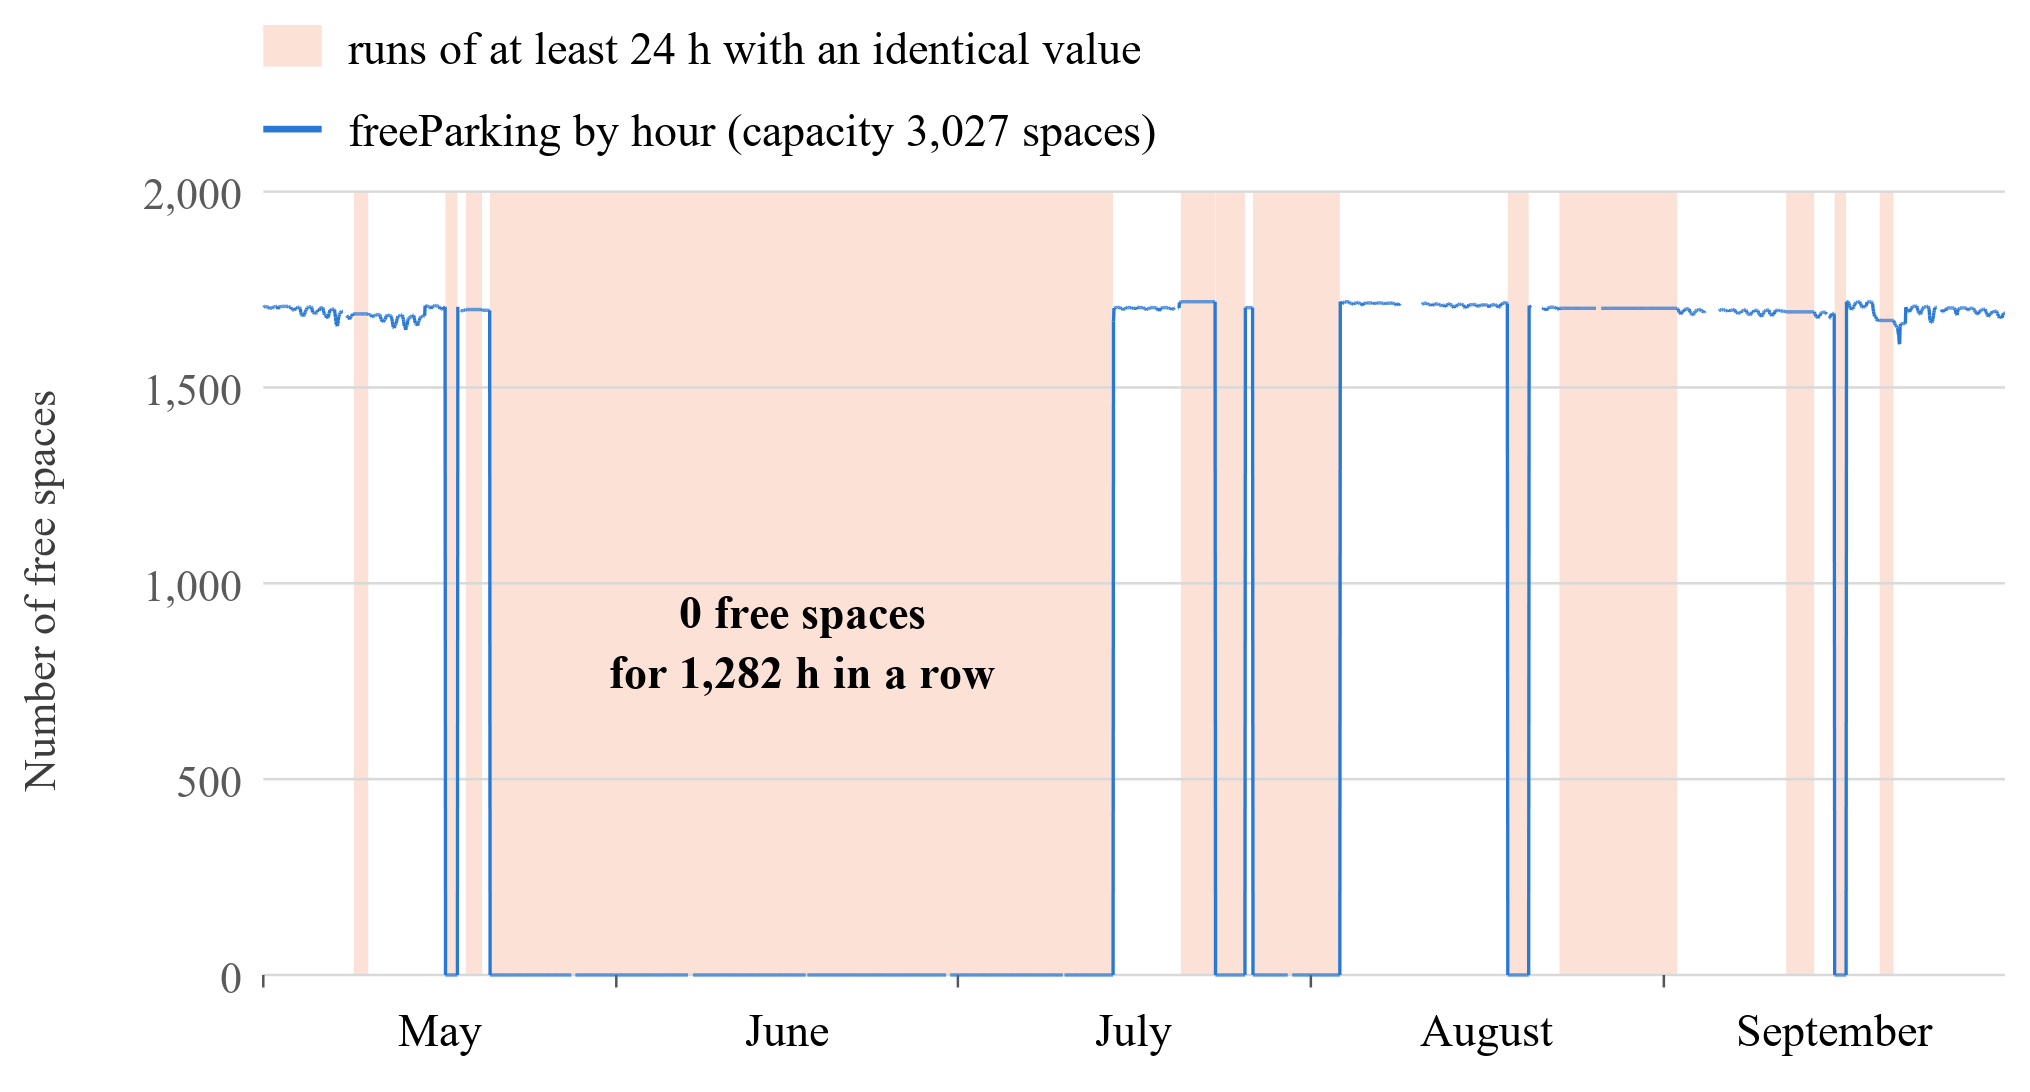
\includegraphics[width=0.9\linewidth]{image/fig1_id80.png}
  \caption{Hourly number of free spaces at car park ID 80 (capacity 3,027)}
  \label{fig:1}
\end{figure}

The effect of frozen runs on the reference measures is shown in Table 6 and Figure 2. Excluding the runs lowers occupancy by rows by 1.9--3.5 pp and June capacity-weighted occupancy by 11 pp. Peak hours and August's position as the month of lowest occupancy do not change. At \emph{L} = 12, 10,741 rows are excluded and the conclusions stay the same. The June peak under P1 is created mainly by the zero run of ID 80: excluding this car park alone gives 53.2\% for June, and under P1-S June does not stand out from neighbouring months.

\begin{table}[htbp]
  \caption{Reference measures under rules P1 and P1-S}
  \label{tab:6}
  \centering\small
  \begin{tabular}{p{\dimexpr 0.140\linewidth-2\tabcolsep\relax}p{\dimexpr 0.130\linewidth-2\tabcolsep\relax}p{\dimexpr 0.220\linewidth-2\tabcolsep\relax}p{\dimexpr 0.230\linewidth-2\tabcolsep\relax}p{\dimexpr 0.280\linewidth-2\tabcolsep\relax}}
    \hline
    \textbf{Month} & \textbf{Rows excluded} & \textbf{Occupancy by rows, \%} & \textbf{Capacity-weighted occupancy, \%} & \textbf{Busiest car park} \\ \hline
    May & 2,068 & 54.5 $\to$ 52.5 & 57.6 $\to$ 52.5 & 15 $\to$ 55 (77.4\%) \\
    June & 2,882 & 53.7 $\to$ 51.3 & 63.8 $\to$ 52.8 & 15, 80 $\to$ 55 (75.8\%) \\
    July & 2,050 & 49.6 $\to$ 46.1 & 57.7 $\to$ 47.8 & 15 $\to$ 55 (76.7\%) \\
    August & 1,649 & 44.4 $\to$ 41.6 & 47.1 $\to$ 43.0 & 15 $\to$ 55 (72.6\%) \\
    September & 1,502 & 53.1 $\to$ 51.2 & 52.9 $\to$ 51.1 & 15 $\to$ 55 (77.8\%) \\
    \hline
  \end{tabular}
\end{table}

\begin{figure}[htbp]
  \centering
  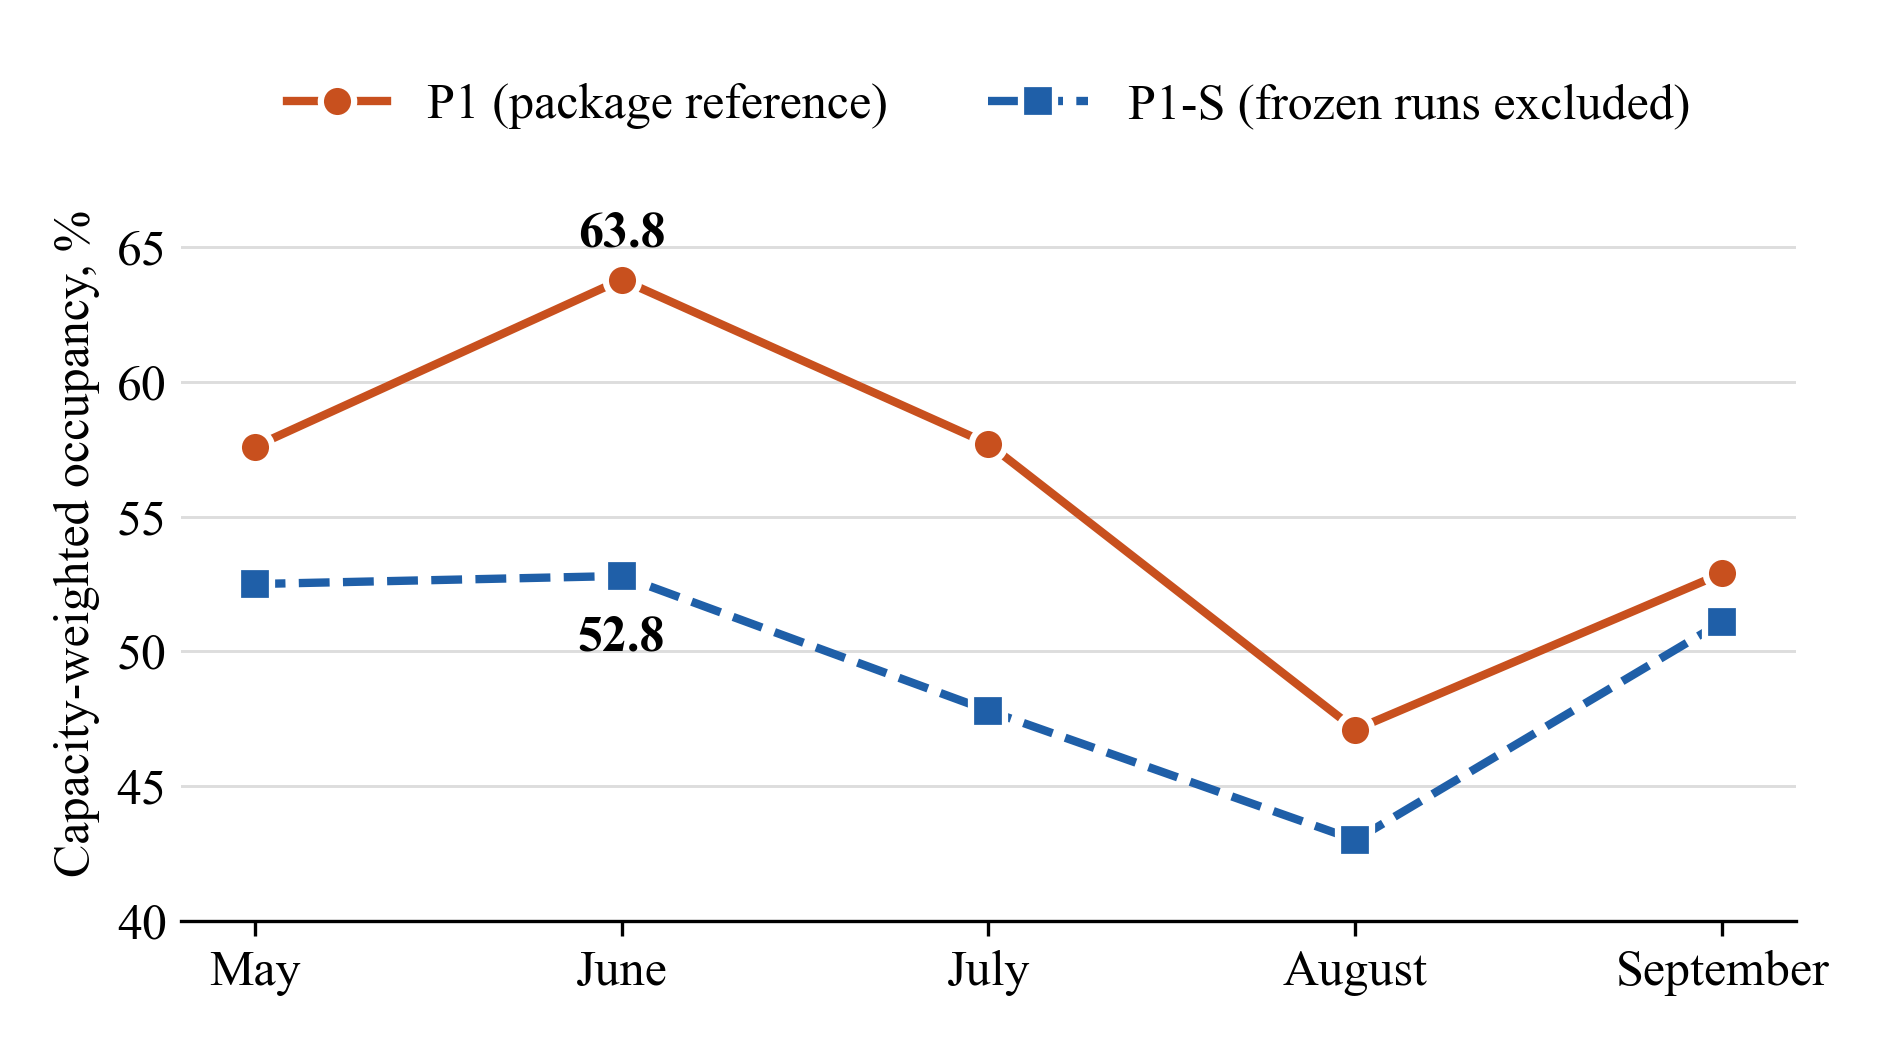
\includegraphics[width=0.9\linewidth]{image/fig2_occupancy.png}
  \caption{Capacity-weighted occupancy under rules P1 and P1-S}
  \label{fig:2}
\end{figure}

\subsection{Sensitivity of references}

Table 7 summarises the sensitivity analysis. All means, standard deviations, and shares (25 of 40 fractional references) fail even under rounding to four decimals; medians and quartiles are integers and are unaffected. The quantile method does not change the quartiles of the whole dataset but does change the integer outlier count, which is compared exactly even though the question does not state the method.

\begin{table}[htbp]
  \caption{Broken references under typical deviations}
  \label{tab:7}
  \centering\small
  \begin{tabular}{p{\dimexpr 0.420\linewidth-2\tabcolsep\relax}p{\dimexpr 0.270\linewidth-2\tabcolsep\relax}p{\dimexpr 0.310\linewidth-2\tabcolsep\relax}}
    \hline
    \textbf{Deviation} & \textbf{Broken references} & \textbf{Size of discrepancy} \\ \hline
    Rounding to 2--4 decimals at tolerance 10$^{-6}$ & 25 of 40 fractional & Up to 5$\cdot$10$^{-5}$ at 4 decimals \\
    Shares as percentages with two decimals & 15 of 15 shares & Up to 5$\cdot$10$^{-5}$ \\
    ddof = 0 instead of 1 & 5 of 5 SD & 0.003--0.007 spaces \\
    Filter ``not below zero'' instead of P1 & n, mean, median, SD, occupancy & Median +1; occupancy $-$1.3 to $-$1.4 pp \\
    No filtering & Almost all & Occupancy 82--84\% instead of 44--54\%; median $-$1 \\
    Other quantile method for Q1 and Q3 & None & Identical under three methods \\
    Other quantile method for group interquartile range & 5 of 5 outlier counts & From $\pm$1 to $\pm$3 \\
    Algebraically equal occupancy formula (\emph{c} $-$ \emph{f})/\emph{c} & 3 of 5 outlier counts & From $-$1 to +21 \\
    Interquartile range without grouping by car park & 5 of 5 outlier counts & 0 instead of 199--472 \\
    \hline
  \end{tabular}
\end{table}

Two types of references are unreliable in substance. Under P1 the busiest car park is ID 15, with a constant zero (in June, tied with ID 80). The May peak hour beats its neighbour by only 0.13 pp (68.10\% versus 67.97\%), and the August peak hour by 0.25 pp.

\subsection{Structure of missing values}

Among the 20 working EMT car parks, $-$1 takes up 4.86\% of rows, and almost all of these gaps are system-wide: in 178 of 3,672 date-hours, $-$1 appears at all 20 car parks at once, while partial failures occur in only two date-hours. Among the 10 working non-EMT car parks the share of $-$1 is 0.20\%. Failures are unevenly distributed by month (20, 21, 18, 78, and 41 h; 44\% in August, including the window on 26 August from 04:00 to 09:00 when all 82 car parks are unavailable) and occur more often at night (10--13 cases per hour label for hours 02--08, versus 3--5 in the evening). Monthly means barely shift: the mean of the 24 hourly means differs from the mean by rows by no more than 0.28 pp.

\subsection{Error in a reference field}

ID 32 accounts for 672 of the 685 capacity overruns. With a declared 212 spaces, the number of free spaces reaches 231. Overruns are stable (119 to 146 per month) and concentrated between 22:00 and 09:00, peaking at 04:00--06:00, when the car park empties, which points to an understated capacity. P1 removes 18.3\% of the non-negative rows of ID 32, and these are precisely its emptiest hours. Its occupancy is therefore 33.0\% under P1 and 26.9\% if values are clipped to capacity.

\subsection{Seasonality}

Table 8 gives the results of coverage control. Under every method August remains the month of lowest occupancy, 4.2--5.2 pp below the next lowest month, July. At 25 of the 27 stable car parks, August occupancy is below their own mean for the other months (two-sided sign test, \emph{p} $\approx$ 6$\cdot$10$^{-6}$; descriptive only, as car parks are not independent), and at 21 car parks August is the minimum of the five months. The weekly cycle of these car parks almost disappears in August: weekdays exceed Sundays by 1.7 pp versus 6.0--9.4 pp in other months. The package's warning that differences between months are explained by coverage is not confirmed for August.

\begin{table}[htbp]
  \caption{Mean occupancy under different coverage controls, \%}
  \label{tab:8}
  \centering\small
  \begin{tabular}{p{\dimexpr 0.400\linewidth-2\tabcolsep\relax}p{\dimexpr 0.120\linewidth-2\tabcolsep\relax}p{\dimexpr 0.120\linewidth-2\tabcolsep\relax}p{\dimexpr 0.120\linewidth-2\tabcolsep\relax}p{\dimexpr 0.120\linewidth-2\tabcolsep\relax}p{\dimexpr 0.120\linewidth-2\tabcolsep\relax}}
    \hline
    \textbf{Method} & \textbf{May} & \textbf{June} & \textbf{July} & \textbf{August} & \textbf{September} \\ \hline
    P1, by rows & 54.5 & 53.7 & 49.6 & 44.4 & 53.1 \\
    27 stable car parks, equal weight & 52.1 & 50.0 & 46.0 & 41.6 & 51.4 \\
    Balanced panel & 55.2 & 52.2 & 48.2 & 43.1 & 54.0 \\
    Day of week $\times$ hour standardisation & 52.1 & 49.7 & 45.7 & 41.5 & 51.2 \\
    P1-S & 52.5 & 51.3 & 46.1 & 41.6 & 51.2 \\
    \hline
  \end{tabular}
\end{table}

\subsection{LLMs and agents on the reference questions}

Agents answered 71--85 of the 85 questions correctly, and models without tools 5--10 (Table 9). The 48 correct answers without tools are trivial: 29 give the row count, which the prompt itself stated, 8 a zero count, and 11 name ID 15, whose zero readings are visible in the first rows. Accepting the P1-S alternative changed no score: no agent excluded frozen sensors on its own.

\begin{table}[htbp]
  \caption{Correct answers out of 85}
  \label{tab:9}
  \centering\small
  \begin{tabular}{p{\dimexpr 0.240\linewidth-2\tabcolsep\relax}p{\dimexpr 0.120\linewidth-2\tabcolsep\relax}p{\dimexpr 0.160\linewidth-2\tabcolsep\relax}p{\dimexpr 0.160\linewidth-2\tabcolsep\relax}p{\dimexpr 0.160\linewidth-2\tabcolsep\relax}p{\dimexpr 0.160\linewidth-2\tabcolsep\relax}}
    \hline
    \textbf{Model} & \textbf{Mode} & \textbf{Package, strict} & \textbf{Package, protocol scoring} & \textbf{Protocol, strict} & \textbf{Protocol, protocol scoring} \\ \hline
    Claude Sonnet 5.5 & LLM & 10 & 10 & 9 & 9 \\
     & Agent & 70 & 77 & 54 & 79 \\
    GPT-6.1 Sol & LLM & 5 & 5 & 5 & 5 \\
     & Agent & 85 & 85 & 59 & 84 \\
    DeepSeek-V4-Pro & LLM & 10 & 10 & 9 & 9 \\
     & Agent & 71 & 71 & 55 & 80 \\
    \hline
  \end{tabular}
\end{table}

Under the protocol condition, strict comparison rejected exactly 25 correct answers of every agent. These are the 25 fractional references that break under rounding to four decimals (Table 7), and the protocol asks for that rounding. Under the package condition GPT-6.1 Sol returned full precision and lost nothing, while Claude Sonnet 5.5 rounded seven answers. An agent needed on average 2.6--2.7 thousand tokens per question with GPT-6.1 Sol, 3.4--12.7 thousand with DeepSeek-V4-Pro, and 18--22 thousand with Claude Sonnet 5.5.

The 34 agent errors fall into four groups (Table 10), and none of them is an error of arithmetic on a well-defined question. 21 errors concern the outlier question alone. Eight answers equal the count obtained with the algebraically equal formula \emph{o} = (\emph{c} $-$ \emph{f})/\emph{c}: in floating point it rounds differently from Eq. (1), and values that lie exactly on an outlier fence in exact arithmetic fall on one side or the other. The size of the effect is shown in Table 11: in July the two formulas give 344 and 365. Exact rational arithmetic gives 342 in July and 465 in August, so the references for these two months are themselves off by 2 and 7.

\begin{table}[htbp]
  \caption{Causes of agent errors (510 agent runs)}
  \label{tab:10}
  \centering\small
  \begin{tabular}{p{\dimexpr 0.560\linewidth-2\tabcolsep\relax}p{\dimexpr 0.120\linewidth-2\tabcolsep\relax}p{\dimexpr 0.320\linewidth-2\tabcolsep\relax}}
    \hline
    \textbf{Cause} & \textbf{Errors} & \textbf{Example} \\ \hline
    Outlier count under the equal formula (\emph{c} $-$ \emph{f})/\emph{c} & 8 & 305 instead of 303 (June) \\
    Rows kept by the IQR rule reported instead of rows flagged & 11 & 21,565 instead of 199 (May) \\
    IQR outliers removed before computing another measure & 7 & Mean 157.49 instead of 188.50 (May) \\
    No final answer: iteration limit or empty message & 8 & --- \\
    \hline
  \end{tabular}
\end{table}

\begin{table}[htbp]
  \caption{Outlier counts under three ways of computing occupancy}
  \label{tab:11}
  \centering\small
  \begin{tabular}{p{\dimexpr 0.200\linewidth-2\tabcolsep\relax}p{\dimexpr 0.300\linewidth-2\tabcolsep\relax}p{\dimexpr 0.250\linewidth-2\tabcolsep\relax}p{\dimexpr 0.250\linewidth-2\tabcolsep\relax}}
    \hline
    \textbf{Month} & \textbf{Reference, Eq. (1)} & \textbf{(\emph{c} $-$ \emph{f})/\emph{c}} & \textbf{Exact arithmetic} \\ \hline
    May & 199 & 200 & 199 \\
    June & 303 & 305 & 303 \\
    July & 344 & 365 & 342 \\
    August & 472 & 468 & 465 \\
    September & 220 & 220 & 220 \\
    \hline
  \end{tabular}
\end{table}

Eighteen errors, 11 of them on the outlier question, come from the wording. The package rule ends with ``IQR and constant values retained'', meaning that outliers are not removed, but DeepSeek-V4-Pro and once Claude Sonnet 5.5 read it as an instruction to apply an IQR filter while keeping constant values. Under the protocol wording no agent applied the filter. The outlier question asks how many rows are ``flagged'' and adds that they ``are retained''; 11 answers gave the number of retained rows, and Claude Sonnet 5.5 explicitly noted the ambiguity before answering.

\subsection{Defect detection by agents}

All 15 reviews produced a report. The models differ much more here than in answering questions (Table 12). GPT-6.1 Sol found all 43 defect--month pairs, including the system-wide failures and the shorter frozen runs at IDs 76, 79, and 9, and gave their dates and effect on the means. Claude Sonnet 5.5 found 24 and DeepSeek-V4-Pro 19: both reliably reported the service value, the car parks without data, and the overruns at ID 32, but rarely the frozen sensors and never the system-wide failures. On average a review took 58 thousand tokens with GPT-6.1 Sol, 127 thousand with DeepSeek-V4-Pro, and 450 thousand with Claude Sonnet 5.5.

\begin{table}[htbp]
  \caption{Checklist defects found in the agent reviews}
  \label{tab:12}
  \centering\small
  \begin{tabular}{p{\dimexpr 0.460\linewidth-2\tabcolsep\relax}p{\dimexpr 0.180\linewidth-2\tabcolsep\relax}p{\dimexpr 0.180\linewidth-2\tabcolsep\relax}p{\dimexpr 0.180\linewidth-2\tabcolsep\relax}}
    \hline
    \textbf{Defect} & \textbf{GPT-6.1 Sol} & \textbf{Claude Sonnet 5.5} & \textbf{DeepSeek-V4-Pro} \\ \hline
    Service value $-$1; car parks with no valid values & 10 / 10 & 10 / 10 & 10 / 10 \\
    Free spaces above capacity at ID 32 & 5 / 5 & 5 / 5 & 5 / 5 \\
    Values below $-$1 at ID 37 & 3 / 3 & 1 / 3 & 2 / 3 \\
    Constant values at IDs 15 and 49 & 10 / 10 & 5 / 10 & 2 / 10 \\
    Zero runs and jumps at ID 80 & 5 / 5 & 3 / 5 & 0 / 5 \\
    Frozen runs at IDs 76, 79, and 9 & 5 / 5 & 0 / 5 & 0 / 5 \\
    System-wide failures & 5 / 5 & 0 / 5 & 0 / 5 \\
    Total & 43 / 43 & 24 / 43 & 19 / 43 \\
    Reports with false defects & 0 / 5 & 5 / 5 & 5 / 5 \\
    \hline
  \end{tabular}
\end{table}

The reviews also contained claims outside the checklist. All three models found the overruns at ID 37 in May and at ID 17 in September, which Table 3 counts only in the total of 685. Claude Sonnet 5.5 and DeepSeek-V4-Pro read isEmtPark as a flag meaning that a car park is empty and reported thousands of ``contradictions'' with the measurements in every month, whereas GPT-6.1 Sol noted that the meaning of the field is not documented and did not call it an error. Both annotators found false claims in all ten reports of Claude Sonnet 5.5 and DeepSeek-V4-Pro and in none of GPT-6.1 Sol; besides isEmtPark, they include ID 15 listed among the car parks without data and gaps in identifier numbering called a defect. Scoring defect detection therefore needs a penalty for false defects as well as a checklist.

\section{Discussion}

\subsection{Interpretation}

A reference answer is meaningful only together with the conventions used to compute it. The package's questions state ddof = 1 and linear interpolation for Q1 and Q3, but not the number of decimals or the quantile method for the group outlier count, and these omissions produce real discrepancies. Stating a convention matters: numpy.std uses ddof = 0 by default and pandas uses ddof = 1, so without the statement two correct implementations would diverge by more than the tolerance. The difference is practically negligible: at \emph{n} $\approx$ 2$\cdot$10$^{4}$ the relative SD discrepancy is about 1/(2\emph{n}) $\approx$ 2.4$\cdot$10$^{-5}$, so the violation here is created by the 10$^{-6}$ tolerance itself.

A reference can be computed without error and still describe an artifact. The answer ``the busiest car park is ID 15'' is correct under P1, although ID 15 shows a constant zero for the whole period, which suggests a probable fault. A system that notices this and excludes the sensor is scored as wrong under strict comparison. Unlike the cases in~\cite{northcutt2021,wretblad2024}, such a reference cannot be corrected, because the true value is not in the data; sensitive measures therefore need dual references under P1 and P1-S.

The experiment shows how much of the measured error belongs to the references rather than to the systems. Every agent error was either a missing answer or tied to the outlier question and the rule wording, and strict comparison alone removed 25 correct answers from each agent under the protocol. A count that compares floating-point values with a threshold is not a well-defined reference: two equal formulas differ by up to 21 rows, and two of the five package values differ from the exact ones. Such counts should be computed in exact arithmetic or accepted within the range of equal formulas.

The ability to detect defects should be scored separately from answer accuracy, since a system can compute every value correctly and still miss that a sensor is frozen. In the experiment the agents answered questions about occupancy and the busiest car park under P1 and almost never mentioned the frozen sensors, although the protocol asked them to: only 2 of 30 answers about the busiest car park did. In the open review GPT-6.1 Sol found all checklist defects and the other two agents about half (Table 12), so a high score on questions does not imply that a system will notice faulty data. Tables 3 and 5 can serve as a checklist for such scoring.

The August decline and the weakening of the weekly cycle are consistent with a seasonal fall in demand during the holiday period, but a causal interpretation requires external data and was not tested here.

\subsection{Evaluation protocol}

For comparing LLMs and AI agents on this dataset we recommend the following:

\begin{enumerate}
  \item include verbatim in the prompt rule P1, ddof = 1, the quantile method (also for group outliers), the requirement to return all ties, the units, and the number of decimals;
  \item compare fractional answers after rounding to four decimals or with a relative tolerance of 2$\cdot$10$^{-4}$, and accept shares both as fractions and as percentages (at a share of 0.42, rounding to four decimals gives a relative error of up to 1.2$\cdot$10$^{-4}$, so a tolerance of 10$^{-4}$ would be too small); this tolerance does not distinguish ddof = 0 from ddof = 1, so compliance should be checked in the solution code;
  \item compare integer counts, hours, and identifiers exactly, and lists as sets; compute counts that compare fractional values with a threshold, such as the outlier count, in exact arithmetic, or accept every count given by equal formulas;
  \item word rules and questions so that ``flagged'' cannot be read as ``retained'' and a statement that values are retained cannot be read as an instruction to filter;
  \item for occupancy and the busiest car park, accept an answer under P1 or under P1-S if frozen sensors were justifiably excluded;
  \item separately score the share of detected defects from Tables 3 and 5 using a checklist with two annotators, and count false defects;
  \item mark the May and August peak-hour questions as small-margin questions and analyse them separately.
\end{enumerate}

\subsection{Limitations}

The audit was carried out by the team that prepared the package, so it is not an external review. AI assistants were used in the work, and the scripts of the first analyses were not preserved; the reported values come from a later re-implementation, audit\_repro.py. We studied one dataset of one series; the five files are similar in size and structure and are not independent, so the sensitivity estimates cannot be transferred to other datasets without checking. Occupancy conclusions refer to the available measurements of 30 of 82 car parks, not to the city's stock. The meaning of $-$1, the hour label, and the time zone are not described on the dataset pages~\cite{emt,madrid}, and reading $-$1 as a missing measurement is an assumption.

The detector threshold was chosen by expert judgement and robustness was checked only at \emph{L} = 12. There is no ground truth for faults: a long constant value may be real (for example, a closed car park). The detector also does not reveal all defects: P1-S retains the readings of ID 80 outside frozen runs, although their reliability is doubtful. The experiment has its own limits. The models were reached through a third-party gateway, so we cannot verify which model versions served the requests. Each question was asked once at temperature 0 and in Russian, so run-to-run variation was not measured. The iteration limit caused 8 of the 34 agent errors, and models without tools saw only 200 rows, so their scores are a lower bound. The two annotators agreed on all 129 defect--report pairs and on all 15 false-claim judgements (Cohen's κ = 1.0); the criteria left little room for judgement, and agreement may be lower with less explicit criteria. The data were published in 2026, which reduces but does not eliminate the risk of their entering training sets~\cite{sainz2023}. The official files may be updated, so all results refer to the recorded hashes.

\section{Conclusions}

We audited the EMT open parking dataset and a package of reference answers for comparing LLMs and AI agents. The technical reproducibility of the package was confirmed: checksums, re-execution, and independent recalculation agree. Reproducibility, however, does not guarantee that a reference is meaningful: two thirds of rows hold a service value, almost half of the spaces have no measurements, 9.6\% of valid rows belong to frozen runs, and frozen sensors determine both the apparent June peak in weighted occupancy and the answer about the busiest car park.

Rounding breaks 25 of 40 fractional references, the ddof correction breaks all five standard deviations, and the choice of quartile method breaks all five outlier counts. The August decline in occupancy was confirmed by all coverage controls. The proposed protocol comprises explicit conventions in the prompt, an adjusted tolerance, exact computation of threshold counts, unambiguous wording, dual references, and separate scoring of defect detection.

The experiment with three LLMs confirmed these effects. Agents with code execution answered 71--85 of 85 questions correctly and models without tools 5--10, but every agent error came from a missing answer, the outlier question, or the rule wording, and strict comparison rejected 25 correct answers of each agent. In answers to questions the agents rarely mentioned frozen sensors; in an open review GPT-6.1 Sol found all 43 checklist defects and the other agents 24 and 19, and only its reports contained no false defects. Future work includes repeated runs, more models and datasets, and a check of the detector on data with labelled faults.

\begin{dataavailability}
The source data are open~\cite{emt,madrid}. The package, including unchanged source files, reference answers, and calculation programs, the audit script audit\_repro.py, the experiment code, and the logs of all experiment runs are available at https://github.com/klinich-1/Analysis-of-structured-data. The script is a later re-implementation: the scripts of the first analyses were not preserved.
\end{dataavailability}

\begin{acknowledgments}
\textbf{Funding:} This research received no external funding. \textbf{Author contributions:} Conceptualisation: T. M. Kizilbaev, K. V. Bagin; methodology: T. V. Novikov, E. E. Golovin; software: K. V. Bagin, E. E. Golovin; validation: T. V. Novikov, R. R. Balapanov; formal analysis: E. E. Golovin, T. M. Kizilbaev; investigation: R. R. Balapanov, K. V. Bagin; data curation: T. M. Kizilbaev, R. R. Balapanov; writing -- original draft: K. V. Bagin, T. V. Novikov; writing -- review and editing: all authors. All authors have read and agreed to the submitted version of the manuscript. \textbf{Use of AI:} The study design, the audit, the analysis of the results, and the manuscript were prepared by the authors, and the reference package by the authors' project team. AI-based assistants were used as follows: Codex (October 2026; the exact model version was not recorded) was used to prepare the package's calculation code, reference answers, report, and reconciliation script, and Claude Opus 5.5 (Anthropic; November 2026) wrote the recalculation script audit\_repro.py and the experiment code and was used to edit the text, translate the manuscript, and check the references. AI-based tools were also used in part of the audit; their logs were not preserved. All code and text produced with the help of AI were checked and edited by the authors. The models evaluated in the experiment are listed in Materials and methods. The authors verified the results and take full responsibility for them.
\end{acknowledgments}

\begin{conflictsofinterest}
The authors declare no conflict of interest. The audited package was prepared by the authors' own project team.
\end{conflictsofinterest}

\putbib[cite]

\makealttitle

} % END \selectlanguage

\end{document}
